\chapter{Ensemble Learning}

\section{Introduction}

Bagging and boosting are two fundamental \textbf{ensemble learning strategies}---methods of combining multiple models to achieve better results than any single model alone. While both create ensembles of models, they differ fundamentally in how they construct and combine these models.

\section{Bagging (Bootstrap Aggregating)}

The main philosophy of bagging is that \textit{``Many independent opinions are better than one''}

Bagging is a simple way to make a noisy model more stable. Imagine you have a wobbly predictor-like a deep decision tree-that can change its mind a lot if the training data changes a little. Instead of trusting a single tree, bagging builds many versions of that model on slightly different views of the data, and then averages their answers (or takes a majority vote for classification). Averaging smooths out the noise, so the final prediction is steadier and usually more accurate.

How do we get those slightly different views? That's where bootstrapping comes in. From the original training set, \textbf{we repeatedly draw new datasets of the same size with replacement (so the same example can appear multiple times, and some examples are left out).} Each bootstrapped dataset trains its own model. Because each model sees a different sample, their mistakes won't line up perfectly—averaging then cancels out a lot of the randomness.

Why does this help? Many models, especially high-variance ones like decision trees, can overfit the quirks of a single dataset. \textbf{Bagging reduces variance by blending many perspectives, without increasing bias too much}. In practice, this often yields a solid accuracy boost and better reliability. A nice side effect is you get out-of-bag estimates: the examples left out of each bootstrap can be used as a built-in validation set to measure performance without a separate hold-out.

\textbf{Bagging isn't magic—if the base model is already very stable (low variance) or consistently biased in the wrong direction, averaging won't fix the core problem.} It also \textbf{costs more compute and can feel less interpretable} since you're dealing with many models instead of one. But as a foundational ensemble idea, bagging is both elegant and powerful—and it's the backbone of methods like Random Forests, which add an extra twist by randomly selecting features, too.

Still, two facts make bagging effective:
\begin{enumerate}
	\item \textbf{Variance reduction by averaging}: Training many models on these different mixes and averaging their predictions smooths out noise (reduces variance), especially for models that change a lot when the data changes (like deep trees).
	\item \textbf{Bootstrap as a population proxy}: Drawing with replacement from ($D$) mimics sampling from the underlying data-generating process via the empirical distribution. This is not perfect independence, but for many learners it's good enough to bring ($\bar h$) close to ($\mathbb{E}_D[h^D(x)]$) in practice, especially for unstable learners (small data perturbations $\to$ large model changes), like deep decision trees.
\end{enumerate}

\subsection{Bias–variance intuition}

\begin{itemize}
	\item Variance: Bagging typically decreases variance because averaging stabilizes predictions.
	\item Bias: Bagging usually does not increase bias, and may slightly reduce it for some learners. But its main win is variance.
	\item Who benefits most? Unstable learners (\eg trees, k-NN with small ($k$)) benefit a lot. Stable learners (\eg linear/ridge regression) benefit less, though averaging can still help in noisy regimes.
\end{itemize}

Their are some costs: 
\begin{itemize}
	\item Interpretability
	\item Computational costs
\end{itemize}

When and why it works (and when it doesn't):
\begin{itemize}
	\item Correlation matters. If base learners are too correlated, variance reduction is limited. This is why Random Forests add feature subsampling at each split to further decorrelate trees, improving over plain bagging of trees.
	\item Computational cost. Training ($M$) models costs ($M\times$) as much compute (though it parallelizes nicely).
	\item Interpretability. An averaged ensemble is harder to interpret than a single model (especially vs. a small tree or linear model). You can mitigate with feature importance, partial dependence, SHAP, and so on., but it's still less transparent.
	\item Diminishing returns in ($M$). Gains flatten as (M) grows because you approach the correlation floor. In practice, tens to a few hundreds of models are often sufficient.
\end{itemize}

% \subsection{Intuition}
% We start with a single training set ($D={(x_i,y_i)}_{i=1}^n$). Instead of hoping for many independent datasets, we \textbf{simulate} them by drawing \textbf{bootstrap samples} ($D_1,\dots,D_M$): each ($D_m$) is formed by sampling ($n$) examples \textbf{with replacement} from ($D$). For each ($D_m$), we fit a base learner ($h_m$) (\eg a decision tree, ridge regression, logistic regression). We then \textbf{aggregate} the models:
% \begin{align*}
% 	\bar{h}(x)=\frac{1}{M}\sum_{m=1}^{M}h_m(x).
% \end{align*}

% If we could draw truly independent datasets ($D^{(1)},\dots,D^{(M)}$) from the population and train ($h^{D^{(m)}}$) on each, then the \textbf{empirical average hypothesis} would converge to the \textbf{theoretical average hypothesis} ($\mathbb{E}_D[h^D(x)]$) as ($M\to\infty$). With bagging, our bootstraps come from the \textbf{empirical distribution} of ($D$), not the population, so they're not independent. 

% \begin{itemize}
% 	\item Each bootstrap sample is just a reshuffled, reweighted version of the same original points.
% 	\item So two bootstrap samples will overlap a lot (they reuse the same observations), unlike two brand-new datasets collected from the real world.
% 	\item In short: they're new mixes of the same ingredients, not new ingredients.
% \end{itemize}


\subsection{How It Works}

\begin{enumerate}
    \item \textbf{Bootstrap sampling}: Create multiple random samples from the training data with replacement. This means some data points appear multiple times in a sample, while others may not appear at all.
    
    \item \textbf{Train in parallel}: Train a separate model on each bootstrap sample independently---models do not communicate with each other.
    
    \item \textbf{Aggregate}: Combine predictions through:
    \begin{itemize}
        \item \textit{Classification}: Majority voting
        \item \textit{Regression}: Averaging
    \end{itemize}
\end{enumerate}

\begin{center}
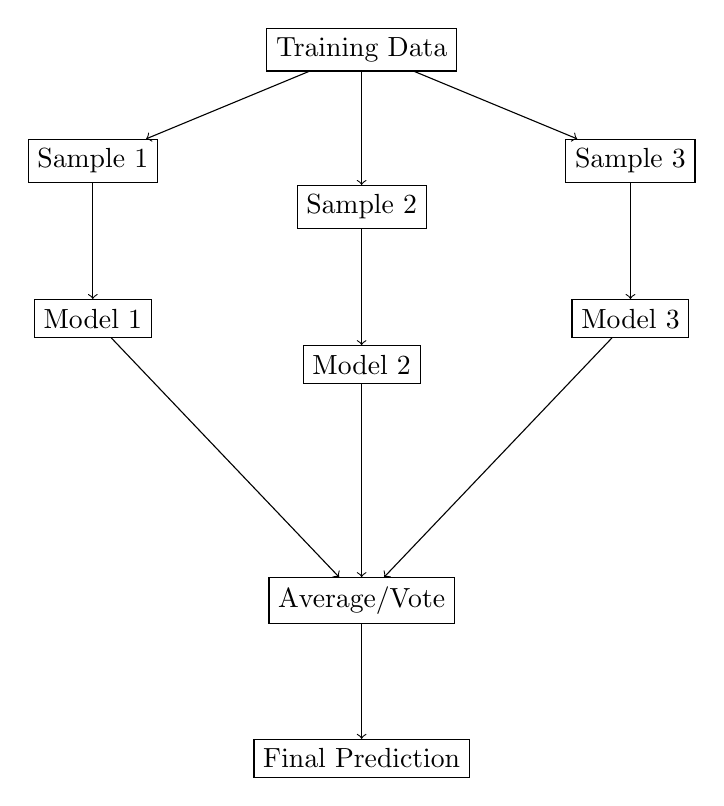
\begin{tikzpicture}[node distance=2cm]
    \node (data) [rectangle, draw] {Training Data};
    \node (sample1) [rectangle, draw, below left of=data, xshift=-2cm] {Sample 1};
    \node (sample2) [rectangle, draw, below of=data] {Sample 2};
    \node (sample3) [rectangle, draw, below right of=data, xshift=2cm] {Sample 3};
    \node (model1) [rectangle, draw, below of=sample1] {Model 1};
    \node (model2) [rectangle, draw, below of=sample2] {Model 2};
    \node (model3) [rectangle, draw, below of=sample3] {Model 3};
    \node (aggregate) [rectangle, draw, below of=model2, yshift=-1cm] {Average/Vote};
    \node (prediction) [rectangle, draw, below of=aggregate] {Final Prediction};
    
    \draw[->] (data) -- (sample1);
    \draw[->] (data) -- (sample2);
    \draw[->] (data) -- (sample3);
    \draw[->] (sample1) -- (model1);
    \draw[->] (sample2) -- (model2);
    \draw[->] (sample3) -- (model3);
    \draw[->] (model1) -- (aggregate);
    \draw[->] (model2) -- (aggregate);
    \draw[->] (model3) -- (aggregate);
    \draw[->] (aggregate) -- (prediction);
\end{tikzpicture}
\end{center}



\paragraph{Mathematical Formulation}

Given a training set $\mathcal{D} = \{(x_i, y_i)\}_{i=1}^{n}$, bagging creates $B$ bootstrap samples and trains models $f_1, f_2, \ldots, f_B$.

\textbf{For regression:}
\begin{equation}
\hat{f}_{\text{bag}}(x) = \frac{1}{B}\sum_{b=1}^{B} f_b(x)
\end{equation}

\textbf{For classification:}
\begin{equation}
	\hat{f}_{\text{bag}}(x) = \argmax_k \sum_{b=1}^{B} \mathbf{1}(f_b(x) = k)
\end{equation}

\begin{itemize}
	\item Key Insight: Each model sees slightly different data, leading to different types of errors. When averaged, errors tend to cancel while correct patterns reinforce each other.
	\item Main Benefit: Reduces \textbf{variance} (overfitting). If one model overfits to peculiar patterns in its sample, other models trained on different samples will not exhibit the same patterns and will balance it out.
\end{itemize}

Examples of Bagging:
\begin{itemize}
    \item Random Forest (bagging with decision trees)
    \item Bagged decision trees
\end{itemize}

\section{Boosting}

The main philosophy of boosting is that \textit{``Learn from your mistakes sequentially''}

\subsection{How It Works}

\begin{enumerate}
    \item \textbf{Start simple}: Train a weak learner (often just slightly better than random guessing)
    
    \item \textbf{Identify mistakes}: Determine which examples the model misclassified
    
    \item \textbf{Focus on failures}: Increase the weight or importance of misclassified examples
    
    \item \textbf{Build the next model}: Train a new model that specifically tries to correct those mistakes
    
    \item \textbf{Repeat}: Continue building models, with each focusing on what previous models struggled with
    
    \item \textbf{Combine}: Sum all models with appropriate weights
\end{enumerate}


\begin{center}
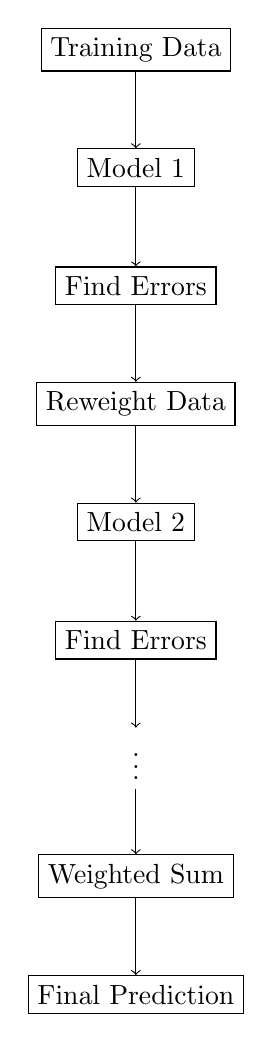
\begin{tikzpicture}[node distance=1.5cm]
    \node (data) [rectangle, draw] {Training Data};
    \node (model1) [rectangle, draw, below of=data] {Model 1};
    \node (error1) [rectangle, draw, below of=model1] {Find Errors};
    \node (weight1) [rectangle, draw, below of=error1] {Reweight Data};
    \node (model2) [rectangle, draw, below of=weight1] {Model 2};
    \node (error2) [rectangle, draw, below of=model2] {Find Errors};
    \node (dots) [below of=error2] {$\vdots$};
    \node (combine) [rectangle, draw, below of=dots] {Weighted Sum};
    \node (prediction) [rectangle, draw, below of=combine] {Final Prediction};
    
    \draw[->] (data) -- (model1);
    \draw[->] (model1) -- (error1);
    \draw[->] (error1) -- (weight1);
    \draw[->] (weight1) -- (model2);
    \draw[->] (model2) -- (error2);
    \draw[->] (error2) -- (dots);
    \draw[->] (dots) -- (combine);
    \draw[->] (combine) -- (prediction);
\end{tikzpicture}
\end{center}

\subsection{Mathematical Formulation}

The final model is a weighted sum of weak learners:

\begin{equation}
F(x) = \sum_{m=1}^{M} \alpha_m f_m(x)
\end{equation}

where $\alpha_m$ is the weight for model $m$, and $f_m$ is the $m$-th weak learner.

\begin{itemize}
	\item Key Insight: Instead of independent models, you build a team where each member specializes in fixing specific weaknesses of the ensemble.
	\item Main Benefit: Reduces \textbf{bias} (underfitting). By sequentially focusing on difficult examples, you build a more accurate overall model.
\end{itemize}

\subsection{AdaBoost}

The most popular boosting algorithm is \textit{AdaBoost}, so-called because it is ``adaptive.'' AdaBoost is extremely simple to use and implement (far simpler than SVMs), and often gives very effective results. There is tremendous flexibility in the choice of weak classifier as well. Boosting is a specific example of a general class of learning algorithms called ensemble methods, which attempt to build better learning algorithms by combining multiple simpler algorithms.

Suppose we are given training data $\{(\rvx_i, y_i)\}^N_{i=1}$, where $\rvx_i \in \mathbb{R}^K$ and $y_i \in \left\{-1, 1\right\}$. And suppose we are given a (potentially large) number of weak classifiers, denoted $f_m(\rvx) \in \left\{-1, 1\right\}$, and a \textbf{0-1} loss function $I$, defined as
\begin{align*}
	I(f_m(\rvx), y) = \begin{cases}
		0&\text{ if } f_m(\rvx_i)=y_i\\
		1&\text{ if } f_m(\rvx_i)\neq y_i
	\end{cases}
\end{align*}
\begin{itemize}
	\item $I=0$ if prediction equals the truth ( $\hat{y}=y$)
	\item $I=1$ if prediction is wrong ( $\hat{y}\neq y$)
\end{itemize}

AdaBoost aims to build a strong classifier by combining many weak ones. It does this in rounds $m=1,2,\dots,M$ :

\begin{enumerate}
	\item Give every training example the same weight. Every sample is equally important at the beginning.
	\item Fit a \textit{weak learner} $f_m$ on the weighted data
	\item Compute how good it is: measure its \textit{weighted error} of weak learner, $e_m$. 
		\begin{align*}
			e_m = \sum_{i=1}^{N}w_i^m \cdot I(f_m(\rvx_i), y_i),
		\end{align*}
		where $w_i^m$ is the current example weight. 
		\begin{itemize}
			\item This measures how many (weighted) mistakes that stump/tree makes this round.
		\end{itemize}
	\item Compute $\alpha_m$, which is the \textit{vote weight} (strength) assigned to that weak learner when forming the final ensemble: 
		\begin{align*}
			\alpha_m = \frac{1}{2}\ln \left(\frac{1-e_m}{e_m}\right).
		\end{align*}
		\begin{itemize}
			\item minimizing the weighted exponential loss for fixed $f_m$.
			\item bigger when the error $e_m$ is smaller
			\item As $e_m\to 0$, $\alpha_m\to \infty$.
			\item As $e_m\to 1$, $\alpha_m\to -\infty$.
		\end{itemize}
	\item Repeat: fit the next weak learner on the reweighted data, and so on.
		\begin{align*}
			w_i^{(m+1)}\propto w_i^{(m)}\cdot \exp(-\alpha_m y_i f_m(\rvx_i)).
		\end{align*}
\end{enumerate}

After learning, the final classifier is based on a linear combination of the weak classifiers:
\begin{align*}
	F(\rvx) = \sum_{m=1}^M \alpha_mf_m(\rvx).
\end{align*}
If more of the strong (high-$\alpha$) weak learners say $+1$ than $-1$, the final answer is $+1$, etc.

This is why it's called \textbf{adaptive:} each new weak learner adapts to the mistakes of the previous ones by focusing more weight on hard examples.



% \textbf{AdaBoost algorithm:}
% \begin{align}
% \text{Initialize: } & w_i^{(1)} = \frac{1}{n}, \quad i = 1, \ldots, n \\
% \text{For } m &= 1 \text{ to } M: \\
% & \text{1. Train } f_m \text{ on weighted data} \\
% & \text{2. Compute error: } \epsilon_m = \sum_{i=1}^{n} w_i^{(m)} \mathbf{1}(f_m(x_i) \neq y_i) \\
% & \text{3. Compute weight: } \alpha_m = \frac{1}{2}\log\left(\frac{1-\epsilon_m}{\epsilon_m}\right) \\
% & \text{4. Update weights: } w_i^{(m+1)} = w_i^{(m)} \exp(-\alpha_m y_i f_m(x_i))
% \end{align}

Examples:
\begin{itemize}
    \item AdaBoost (Adaptive Boosting)
    \item Gradient Boosting Machines (GBM)
    \item XGBoost (Extreme Gradient Boosting)
    \item LightGBM
    \item CatBoost
\end{itemize}

\section{Comparison of Bagging and Boosting}

\begin{table}[h]
\centering
\begin{tabular}{@{}lll@{}}
\toprule
\textbf{Aspect} & \textbf{Bagging} & \textbf{Boosting} \\ 
\midrule
Training & Parallel (all at once) & Sequential (one after another) \\
Model focus & Random sample & Previous errors \\
Main strength & Reduces variance & Reduces bias \\
Speed & Faster (parallelizable) & Slower (sequential) \\
Overfitting risk & Low & Higher (requires tuning) \\
Data weighting & Equal for all samples & Dynamic (hard examples weighted more) \\
Independence & Models are independent & Models are dependent \\
\bottomrule
\end{tabular}
\caption{Comparison of Bagging and Boosting}
\end{table}

\subsection{Bias-Variance Tradeoff}

\subsection{Bagging}
Primarily reduces \textbf{variance} by averaging predictions:
\begin{equation}
\text{Var}(\hat{f}_{\text{bag}}) \approx \frac{\sigma^2}{B}
\end{equation}
where $\sigma^2$ is the variance of individual models and $B$ is the number of models.

\subsection{Boosting}
Primarily reduces \textbf{bias} by iteratively fitting residuals:
\begin{equation}
r_i^{(m)} = y_i - F_{m-1}(x_i)
\end{equation}
where $r_i^{(m)}$ is the residual for observation $i$ at iteration $m$.

\subsection{Use Bagging When:}
\begin{itemize}
    \item Your model tends to overfit (high variance)
    \item You need stability and robustness
    \item You can leverage parallel computing
    \item You want simpler hyperparameter tuning
    \item Interpretability is important
\end{itemize}

\subsection{Use Boosting When:}
\begin{itemize}
    \item You need maximum predictive accuracy
    \item Your base models are too simple (high bias)
    \item You're willing to invest time in careful tuning
    \item You can afford sequential training time
    \item You have sufficient data to avoid overfitting
\end{itemize}

Both bagging and boosting leverage the principle that \textbf{diverse perspectives make better decisions}. They achieve diversity through different mechanisms:

\begin{itemize}
    \item \textbf{Bagging}: Creates diversity through random sampling (variance reduction)
    \item \textbf{Boosting}: Creates diversity through sequential error correction (bias reduction)
\end{itemize}

The choice between them depends on your specific problem, computational resources, and whether your primary concern is reducing variance or bias in your models.


\section{Random Forest}

Think of Random Forest as a ``wisdom of the crowds'' approach to making predictions.

The core idea: Instead of relying on one decision tree to make predictions, you create a whole forest of them (often hundreds) and let them vote on the answer.

\begin{itemize}
	\item You create many decision trees, but each one is trained on a slightly different random sample of your data
	\item Each tree also only looks at a random subset of features when making splits
	\item When you need a prediction, all trees vote, and you take the majority vote (for classification) or average (for regression)
\end{itemize}

\section{Gradient Boosting}

% Similar to AdaBoost, \textit{gradient boosting} is an ensemble method that combines multiple weak learners (such as decision trees) into a strong learner. Also, similar to AdaBoost (and in contrast to Bagging), gradient boosting is a sequential (rather than parallel) algorithm – it is powerful but rather expensive to train.

% In contrast to AdaBoost, we do not adjust the weights for the training examples that have been either misclassified or correctly classified. Also, we do not compute a weight for each model in the sequential gradient boosting ensemble. Instead, in gradient boosting, we \textit{optimize a differentiable loss function} (\eg mean-squared-error for regression or negative log-likelihood for classification) of a weak learner via consecutive rounds of boosting. The output of gradient boosting is an additive models of multiple weak learners (we do not apply majority voting to the ensemble of models like AdaBoost).

% Note that in gradient boosting, we may use decision trees (the most common base learning algorithm for gradient boosting is in fact a decision tree algorithm), but we do not necessarily use decision tree stumps. The first model in gradient boosting is basically just a decision tree's root node (on which we do majority voting in classification or averaging in regression). The consequent models in gradient boosting are deeper decision trees. The depth is usually determined by the practitioner. Values like 8 or 32 are common, depending on the complexity of the dataset/difficulty of the task.

% Conceptually, the main idea behind gradient boosting can be summarized via the following three steps:
% \begin{enumerate}
% 	\item Construct a base tree (just the root node)
% 	\item Build next tree based on errors of the previous tree
% 	\item Combine tree from step 1 with trees from step 2. Go to step 2.
% \end{enumerate}

% Build a strong predictor by stacking many tiny corrections: start with a simple guess, then repeatedly add small models that fix what's still wrong.

% \begin{itemize}
% 	\item Start simple: Make an initial prediction for every data point (\eg the average target value).
% 	\item Look at what you got wrong: Compute the residuals = (true − predicted).
% 	\item For classification, this error is the negative gradient of the loss (that's the "gradient" in gradient boosting).
% 	\item Learn to fix the errors: Train a small, weak model (usually a shallow decision tree) to predict those residuals.
% 	\item Add a small step: Add a fraction (the learning rate) of that weak model to your running prediction.
% 	\item Repeat: Recompute the residuals with the improved predictions, fit another small tree to those, add it in, and so on.
% \end{itemize}

% After ($M$) rounds you have:
% \begin{align*}
% 	\hat{y}(x) = f_0(x) + \nu \cdot h_1(x) + \nu \cdot h_2(x) + \cdots + \nu \cdot h_M(x)
% \end{align*}
% where ($f_0$) is the initial guess, each ($h_m$) is a small tree trained to fix current mistakes, and ($\nu$) is the learning rate (\eg 0.1).

% \begin{itemize}
% 	\item Targets: $[3, 5, 7]$.
% 	\item Initial guess: mean = 5 → predictions $[5, 5, 5]$.
% 	\item Residuals: $[-2, 0, +2]$.
% 	\item Fit a tiny tree to map features → residuals (learns left points are low, right points are high).
% 	\item Add a small step (say 0.5$\times$ tree output) to your predictions.
% 	\item Recompute residuals and repeat. Each round chips away at what's still wrong.
% \end{itemize}

Gradient Boosting is one of the most powerful and widely-used machine learning algorithms. It builds an ensemble of weak learners (typically decision trees) sequentially, where each new model corrects the errors of the previous ones by moving in the direction of the gradient of the loss function.

\begin{itemize}
\item Key Insight: While traditional boosting focuses on misclassified samples, \textbf{Gradient Boosting} takes a more general approach: it fits new models to the \textit{residuals} (errors) of the ensemble, following the negative gradient of a loss function. This makes it extremely flexible and applicable to various problems.

\item The Analogy: Think of gradient boosting as a student improving their test score:
\begin{enumerate}
    \item Take a practice test (first model makes predictions)
    \item Review mistakes (calculate residuals/errors)
    \item Study specifically to fix those mistakes (train new model on residuals)
    \item Take another test (add new model to ensemble)
    \item Repeat until mastery (continue until convergence)
\end{enumerate}
Each iteration focuses on what you got wrong, gradually improving overall performance.
\end{itemize}


\subsection{Mathematical Foundation}

Gradient boosting is fundamentally an optimization algorithm in function space. We want to find a function $F(x)$ that minimizes expected loss:

\begin{equation}
F^* = \underset{F}{\text{argmin}} \, \mathbb{E}_{x,y}[L(y, F(x))]
\end{equation}

where $L(y, F(x))$ is a differentiable loss function.

\begin{enumerate}
    \item \textbf{Initialize} with a constant prediction:
    \begin{equation}
    F_0(x) = \underset{\gamma}{\text{argmin}} \sum_{i=1}^{n} L(y_i, \gamma)
    \end{equation}
    
    \item \textbf{For each iteration} $m = 1$ to $M$:
    
    \begin{enumerate}
        \item \textbf{Compute pseudo-residuals} (negative gradient):
        \begin{equation}
        r_{im} = -\left[\frac{\partial L(y_i, F(x_i))}{\partial F(x_i)}\right]_{F=F_{m-1}}
        \end{equation}
        
        \item \textbf{Fit a weak learner} $h_m(x)$ to predict the residuals $r_{im}$
        
        \item \textbf{Compute optimal step size} (line search):
        \begin{equation}
        \gamma_m = \underset{\gamma}{\text{argmin}} \sum_{i=1}^{n} L(y_i, F_{m-1}(x_i) + \gamma h_m(x_i))
        \end{equation}
        
        \item \textbf{Update the model}:
        \begin{equation}
        F_m(x) = F_{m-1}(x) + \nu \cdot \gamma_m h_m(x)
        \end{equation}
        where $\nu$ is the learning rate (typically $0.01$ to $0.3$)
    \end{enumerate}
    
    \item \textbf{Final model}:
    \begin{equation}
    F_M(x) = F_0(x) + \nu \sum_{m=1}^{M} \gamma_m h_m(x)
    \end{equation}
\end{enumerate}

\subsection{The Gradient Descent Connection}

Gradient boosting performs \textbf{gradient descent in function space}:

\begin{center}
\begin{tabular}{ll}
\toprule
\textbf{Parameter Space} & \textbf{Function Space} \\
\midrule
Parameters: $\theta$ & Function: $F(x)$ \\
Update: $\theta_{t+1} = \theta_t - \eta \nabla_\theta L$ & Update: $F_m = F_{m-1} - \nu \nabla_F L$ \\
Gradient: $\nabla_\theta L$ & Gradient: residuals $r_{im}$ \\
Step size: $\eta$ & Learning rate: $\nu$ \\
\bottomrule
\end{tabular}
\end{center}

\section{Loss Functions}

Different loss functions lead to different gradient boosting variants:

\subsection{Regression Problems}

\textbf{1. Squared Error (L2 Loss)}
\begin{align}
L(y, F(x)) &= \frac{1}{2}(y - F(x))^2 \\
\text{Gradient: } -\frac{\partial L}{\partial F} &= y - F(x) \quad \text{(residuals)}
\end{align}

\textbf{2. Absolute Error (L1 Loss)}
\begin{align}
L(y, F(x)) &= |y - F(x)| \\
\text{Gradient: } -\frac{\partial L}{\partial F} &= \text{sign}(y - F(x))
\end{align}

\textbf{3. Huber Loss} (robust to outliers)
\begin{equation}
L_\delta(y, F(x)) = \begin{cases}
\frac{1}{2}(y - F(x))^2 & \text{if } |y - F(x)| \leq \delta \\
\delta(|y - F(x)| - \frac{1}{2}\delta) & \text{otherwise}
\end{cases}
\end{equation}

\subsection{Classification Problems}

\textbf{Binary Classification (Log Loss)}
\begin{align}
L(y, F(x)) &= \log(1 + e^{-2yF(x)}) \quad y \in \{-1, +1\} \\
\text{Gradient: } -\frac{\partial L}{\partial F} &= \frac{2y}{1 + e^{2yF(x)}}
\end{align}

\textbf{Multi-class Classification (Softmax)}
\begin{align}
L(y, \mathbf{F}(x)) &= -\sum_{k=1}^{K} y_k \log p_k(x) \\
\text{where } p_k(x) &= \frac{e^{F_k(x)}}{\sum_{j=1}^{K} e^{F_j(x)}}
\end{align}

\section{Key Hyperparameters}

\subsection{Learning Rate ($\nu$)}

Controls the contribution of each tree:
\begin{equation}
F_m(x) = F_{m-1}(x) + \nu \cdot h_m(x)
\end{equation}

\begin{itemize}
    \item \textbf{Small $\nu$ (0.01-0.1)}: More trees needed, better generalization, slower training
    \item \textbf{Large $\nu$ (0.3-1.0)}: Fewer trees needed, faster training, higher overfitting risk
\end{itemize}

\textbf{Rule of thumb}: Lower learning rate with more trees often works best.

\subsection{Number of Trees ($M$)}

\begin{itemize}
    \item More trees generally improve training performance
    \item Use cross-validation or early stopping to prevent overfitting
    \item Typical range: 100-1000 trees
\end{itemize}

\subsection{Tree Depth (max\_depth)}

\begin{itemize}
    \item \textbf{Shallow trees (3-6)}: Less overfitting, faster training, good for most problems
    \item \textbf{Deep trees (8-12)}: Can capture complex interactions, higher overfitting risk
\end{itemize}

\subsection{Subsampling}

Sample a fraction of training data for each tree:
\begin{itemize}
    \item Reduces overfitting
    \item Speeds up training
    \item Typical values: 0.5-0.8
    \item When $< 1.0$, called \textbf{Stochastic Gradient Boosting}
\end{itemize}

\subsection{Feature Subsampling}

Sample features (like Random Forest):
\begin{itemize}
    \item \textbf{colsample\_bytree}: Fraction of features per tree
    \item \textbf{colsample\_bylevel}: Fraction of features per tree level
    \item Reduces correlation between trees
\end{itemize}

\section{Regularization Techniques}

\subsection{Shrinkage (Learning Rate)}

Already covered - the most important regularization:
\begin{equation}
F_m(x) = F_{m-1}(x) + \nu \sum_{m=1}^{M} h_m(x), \quad 0 < \nu \leq 1
\end{equation}

\subsection{Tree Constraints}

\begin{itemize}
    \item \textbf{max\_depth}: Limit tree depth
    \item \textbf{min\_samples\_split}: Minimum samples to split a node
    \item \textbf{min\_samples\_leaf}: Minimum samples in leaf nodes
    \item \textbf{max\_features}: Maximum features to consider
\end{itemize}

\subsection{Early Stopping}

Monitor validation performance and stop when it degrades:
\begin{itemize}
    \item Prevents overfitting automatically
    \item Saves computation time
    \item Requires validation set
\end{itemize}

\section{Practical Algorithm Example}

\begin{algorithm}
\caption{Gradient Boosting for Regression (Squared Loss)}
\begin{algorithmic}[1]
\State \textbf{Input:} Training data $(x_i, y_i)_{i=1}^{n}$, learning rate $\nu$, number of iterations $M$
\State \textbf{Initialize:} $F_0(x) = \bar{y} = \frac{1}{n}\sum_{i=1}^{n} y_i$
\For{$m = 1$ to $M$}
    \State \textbf{Compute residuals:} $r_{im} = y_i - F_{m-1}(x_i)$ for $i = 1, \ldots, n$
    \State \textbf{Fit tree:} Train decision tree $h_m$ on data $(x_i, r_{im})$
    \State \textbf{Update model:} $F_m(x) = F_{m-1}(x) + \nu \cdot h_m(x)$
\EndFor
\State \textbf{Return:} $F_M(x)$
\end{algorithmic}
\end{algorithm}

\section{Gradient Boosting vs Other Methods}

\begin{table}[h]
\centering
\small
\begin{tabular}{@{}llll@{}}
\toprule
\textbf{Aspect} & \textbf{Gradient Boosting} & \textbf{Random Forest} & \textbf{AdaBoost} \\
\midrule
Training & Sequential & Parallel & Sequential \\
Focus & Residuals/Gradients & Random samples & Misclassified samples \\
Loss function & Any differentiable & Fixed (Gini/Entropy) & Exponential \\
Flexibility & Very high & Medium & Low \\
Speed & Slower & Faster & Medium \\
Tuning difficulty & Higher & Lower & Medium \\
Overfitting risk & Medium-High & Low & High \\
Feature importance & Yes & Yes & Limited \\
\bottomrule
\end{tabular}
\caption{Comparison of ensemble methods}
\end{table}

\section{Popular Implementations}

\subsection{XGBoost (Extreme Gradient Boosting)}

Optimized gradient boosting with:
\begin{itemize}
    \item Regularized objective function:
    \begin{equation}
    \text{Obj} = \sum_{i=1}^{n} L(y_i, \hat{y}_i) + \sum_{k=1}^{K} \Omega(f_k)
    \end{equation}
    where $\Omega(f) = \gamma T + \frac{1}{2}\lambda \|\mathbf{w}\|^2$
    \item Second-order Taylor approximation for faster optimization
    \item Parallel tree construction
    \item Cache-aware access patterns
    \item Sparsity-aware algorithm for missing values
\end{itemize}

\subsection{LightGBM}

Microsoft's implementation with:
\begin{itemize}
    \item \textbf{Leaf-wise growth}: Grows trees by leaf instead of level
    \item \textbf{GOSS} (Gradient-based One-Side Sampling): Keeps large gradient instances
    \item \textbf{EFB} (Exclusive Feature Bundling): Reduces feature dimensions
    \item Faster training on large datasets
\end{itemize}

\subsection{CatBoost}

Yandex's implementation with:
\begin{itemize}
    \item Native categorical feature support
    \item Ordered boosting to reduce overfitting
    \item Symmetric trees for faster prediction
    \item Robust to overfitting with minimal tuning
\end{itemize}

\section{Visual Understanding}

\subsection{Sequential Model Building}

\begin{center}
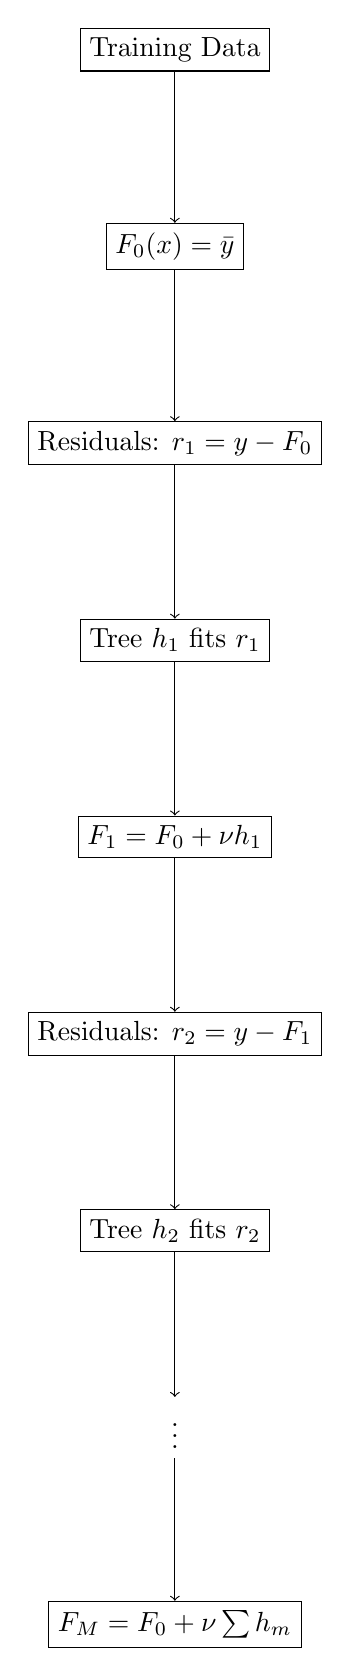
\begin{tikzpicture}[node distance=2.5cm]
    \node (data) [rectangle, draw] {Training Data};
    \node (f0) [rectangle, draw, below of=data] {$F_0(x) = \bar{y}$};
    \node (r1) [rectangle, draw, below of=f0] {Residuals: $r_1 = y - F_0$};
    \node (h1) [rectangle, draw, below of=r1] {Tree $h_1$ fits $r_1$};
    \node (f1) [rectangle, draw, below of=h1] {$F_1 = F_0 + \nu h_1$};
    \node (r2) [rectangle, draw, below of=f1] {Residuals: $r_2 = y - F_1$};
    \node (h2) [rectangle, draw, below of=r2] {Tree $h_2$ fits $r_2$};
    \node (dots) [below of=h2] {$\vdots$};
    \node (final) [rectangle, draw, below of=dots] {$F_M = F_0 + \nu\sum h_m$};
    
    \draw[->] (data) -- (f0);
    \draw[->] (f0) -- (r1);
    \draw[->] (r1) -- (h1);
    \draw[->] (h1) -- (f1);
    \draw[->] (f1) -- (r2);
    \draw[->] (r2) -- (h2);
    \draw[->] (h2) -- (dots);
    \draw[->] (dots) -- (final);
\end{tikzpicture}
\end{center}

\section{Advantages and Disadvantages}

\subsection{Advantages}

\begin{itemize}
    \item \textbf{High accuracy}: Often wins ML competitions
    \item \textbf{Flexibility}: Works with any differentiable loss function
    \item \textbf{Feature importance}: Built-in feature selection
    \item \textbf{Missing values}: Handles them naturally (especially XGBoost)
    \item \textbf{Mixed data types}: Works with numerical and categorical features
    \item \textbf{No feature scaling}: Tree-based, so doesn't require normalization
    \item \textbf{Interpretability}: Can extract feature importance and partial dependence
\end{itemize}

\subsection{Disadvantages}

\begin{itemize}
    \item \textbf{Sequential training}: Cannot parallelize across trees (only within trees)
    \item \textbf{Overfitting}: Requires careful tuning of hyperparameters
    \item \textbf{Training time}: Slower than Random Forest for large datasets
    \item \textbf{Memory intensive}: Stores all trees in memory
    \item \textbf{Sensitive to outliers}: Especially with squared loss
    \item \textbf{Black box}: Less interpretable than single decision trees
\end{itemize}

\section{Best Practices}

\subsection{Hyperparameter Tuning Strategy}

\begin{enumerate}
    \item \textbf{Start with defaults}, establish baseline
    \item \textbf{Tune tree-specific parameters}:
    \begin{itemize}
        \item max\_depth: Start with 3-6
        \item min\_child\_weight: Start with 1
    \end{itemize}
    \item \textbf{Tune learning rate and n\_estimators}:
    \begin{itemize}
        \item Lower learning rate (0.01-0.1)
        \item Increase trees accordingly (use early stopping)
    \end{itemize}
    \item \textbf{Add regularization}:
    \begin{itemize}
        \item Subsampling (0.5-0.8)
        \item Feature subsampling (0.5-0.9)
    \end{itemize}
    \item \textbf{Fine-tune} all parameters together
\end{enumerate}

\subsection{Preventing Overfitting}

\begin{itemize}
    \item Use \textbf{cross-validation} to monitor generalization
    \item Enable \textbf{early stopping} with validation set
    \item Lower the \textbf{learning rate} and increase trees
    \item Use \textbf{subsampling} (both row and column)
    \item Limit \textbf{tree depth} (shallow trees generalize better)
    \item Increase \textbf{regularization} parameters
\end{itemize}

\subsection{When to Use Gradient Boosting}

\textbf{Good for:}
\begin{itemize}
    \item Tabular/structured data
    \item Competitions requiring maximum accuracy
    \item Mixed feature types (numerical + categorical)
    \item When you have time for hyperparameter tuning
    \item Medium-sized datasets (thousands to millions of rows)
\end{itemize}

\textbf{Consider alternatives when:}
\begin{itemize}
    \item Need real-time predictions (use simpler models)
    \item Very large datasets (consider deep learning or linear models)
    \item Need strong interpretability (use linear models or single trees)
    \item Limited computational resources (use Random Forest)
    \item High-dimensional sparse data (use linear models)
\end{itemize}

\section{Example Code Patterns}

\subsection{Sklearn GradientBoostingRegressor}
\begin{verbatim}
from sklearn.ensemble import GradientBoostingRegressor

model = GradientBoostingRegressor(
    n_estimators=100,
    learning_rate=0.1,
    max_depth=3,
    subsample=0.8,
    random_state=42
)
model.fit(X_train, y_train)
\end{verbatim}

\subsection{XGBoost}
\begin{verbatim}
import xgboost as xgb

model = xgb.XGBRegressor(
    n_estimators=100,
    learning_rate=0.1,
    max_depth=3,
    subsample=0.8,
    colsample_bytree=0.8,
    early_stopping_rounds=10
)
model.fit(X_train, y_train, 
          eval_set=[(X_val, y_val)],
          verbose=False)
\end{verbatim}

\section{Summary}

Gradient Boosting is a powerful ensemble technique that:

\begin{enumerate}
    \item Builds models sequentially, each correcting previous errors
    \item Optimizes any differentiable loss function
    \item Combines many weak learners into a strong predictor
    \item Performs gradient descent in function space
    \item Requires careful tuning but delivers excellent results
\end{enumerate}

The key to success with gradient boosting is understanding the bias-variance tradeoff, proper regularization, and systematic hyperparameter tuning.

